\paragraph{IUP03 Visualizar lista de rutinas} \hspace{1cm}\\ 
\label{pant:IUP03} 

\textbf{\textcolor[rgb]{0, 0, 0.545098}{Objetivo}}\\
Esta pantalla permite al Practicante visualizar las rutinas que el Entrenador le ha asignado, las cuales pueden ser rutinas realizadas por el Practicante previamente.\\

\textbf{\textcolor[rgb]{0, 0, 0.545098}{Diseño}}\\
En la figura \ref{fig:IUP03} se muestra la pantalla \nameref{fig:IUP03}, la cual muestra al Practicante las rutinas que el Entrenador le ha asignado, así como también las rutinas realizadas previamente por el Practicante.\\

En la parte inferior derecha se encuentra el botón Regresar, el cual corresponde a regresar al menú principal.

\begin{figure}[H]
	\centering
		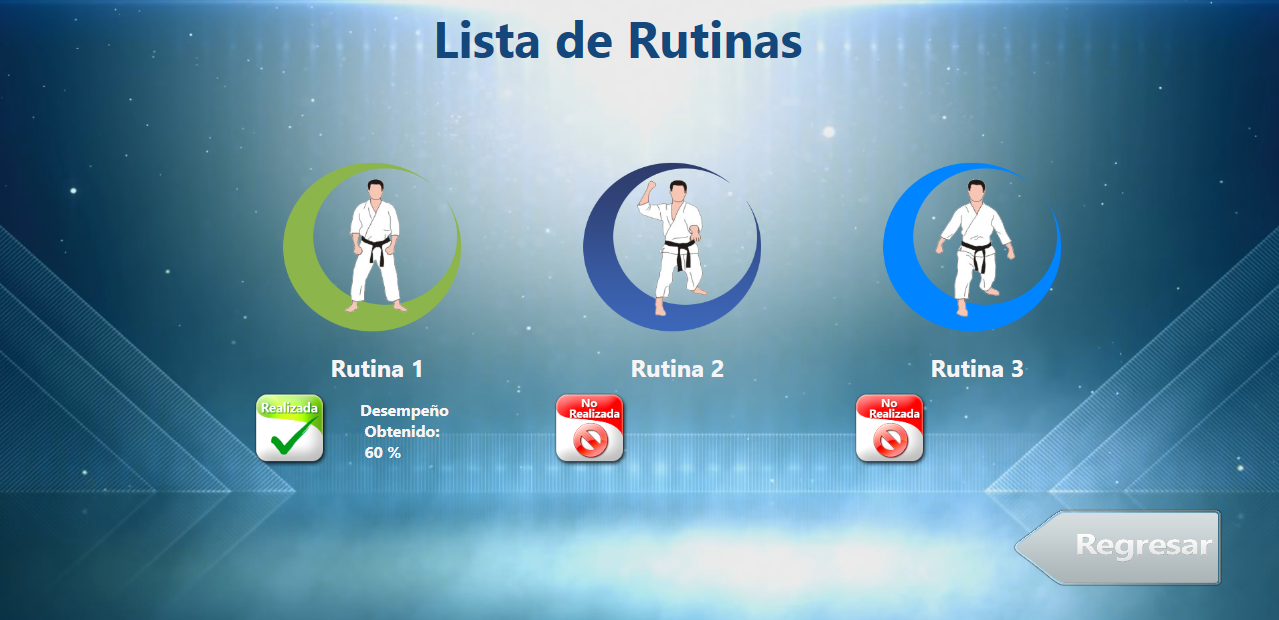
\includegraphics[scale=0.5]{./Figuras/Pantallas/IUP03Visualizar_lista_de_rutinas}
	\caption{IUP03 Visualizar lista de rutinas}
	\label{fig:IUP03}
\end{figure}

\textbf{\textcolor[rgb]{0, 0, 0.545098}{Controles}}
\begin{itemize}
	\item \textbf{\textcolor[rgb]{0, 0, 0.545098}{Lista de Rutinas:}} Permite seleccionar alguna Rutina de entrenamiento. Una vez que se realice una selección, se muestra el menú \nameref{menu:MP02}.
\end{itemize}
\vspace{1em}

\textbf{\textcolor[rgb]{0, 0, 0.545098}{Comandos}}
\begin{itemize}
	\item \textbf{\textcolor[rgb]{0, 0, 0.545098}{Regresar:}} Muestra el menú principal \nameref{menu:MP01}.
\end{itemize}

\vspace{1em}

\textbf{\textcolor[rgb]{0, 0, 0.545098}{Mensajes}}\\
	
\textbf{\nameref{msj:MSG24}}: Se muestra en el menú principal \nameref{menu:MP01} cuando cuando debido a un error de conexión no se muestren los elementos de forma correcta.\\

\clearpage